%%%%%%%%%%%%%%%%%%%%%%%%%%%%%%%%%%%%%%%%%%%%%%%%%%%%%%%%%%%%%%%%%%%%%%%%%%%%%%%%
%2345678901234567890123456789012345678901234567890123456789012345678901234567890
%        1         2         3         4         5         6         7         8

\documentclass[letterpaper, 12 pt]{article}  % Comment this line out
                                                          % if you need a4paper
%\documentclass[a4paper, 10pt, conference]{ieeeconf}      % Use this line for a4
                                                          % paper




% The following packages can be found on http:\\www.ctan.org
\usepackage{graphicx} % for pdf, bitmapped graphics files
\usepackage{bm}
\newcommand{\uvec}[1]{\boldsymbol{\hat{\textbf{#1}}}}
%\usepackage{epsfig} % for postscript graphics files
%\usepackage{mathptmx} % assumes new font selection scheme installed
%\usepackage{times} % assumes new font selection scheme installed
%\usepackage{amsmath} % assumes amsmath package installed
%\usepackage{amssymb}  % assumes amsmath package installed

\title{\LARGE \bf
The Sustainability of AI and Data Centers
}



\author{
Austin Deng\\
\small Institute for Computing in Research \\
\small austin12709@gmail.com
\and  
Mohit Dubey\\
\small Carbon Veda LLC.\\
\small mohit.dubey96@gmail.com
}




\begin{document}



\maketitle
\thispagestyle{empty}
\pagestyle{empty}


%%%%%%%%%%%%%%%%%%%%%%%%%%%%%%%%%%%%%%%%%%%%%%%%%%%%%%%%%%%%%%%%%%%%%%%%%%%%%%%%
\begin{abstract}


With the popularity of AI models like ChatGPT, the demand for data centers and computing resources has grown rapidly. With increased demand for data centers, many concerns over the environmental impact and sustainability of constructing and running data centers have been raised. This paper explores the climate (specifically carbon emissions and water supply) sustainability of running data centers in the Southwestern United States. By projecting future data center power and water demand, this paper investigates the ability for the Southwestern US to develop data centers while maintaining climate and water supply goals. 



\end{abstract}


%%%%%%%%%%%%%%%%%%%%%%%%%%%%%%%%%%%%%%%%%%%%%%%%%%%%%%%%%%%%%%%%%%%%%%%%%%%%%%%%
\section{INTRODUCTION}

The introduction of ChatGPT and other similar large language models has resulted in an explosion of demand for computational power. Data center power consumption is predicted to double by the end of 2030, spurred by AI training and inferencing\cite{GSDemand}. Currently, the US has over 2900 data centers\cite{DCStats}. Each data center draws a significant amount of power and water from its surrounding community\cite{UTDC}. Powering millions of computations and cooling overheating computers means that data centers are constantly consuming electricity and water. Despite innovations in energy efficiency and cooling systems, data centers account for .3\% of global carbon emissions and stress local water supplies\cite{CloudImpact}. 

In order for the United States to meet its goal of a 100\% carbon pollution-free electrical grid, it's essential for US power plants to focus on developing renewable energy sources like solar power and wind power. However, if the demand for electricity significantly outpaces the development of these energy sources, then US power plants will be forced to burn fossil fuels in order to meet demand. Maintaining a reasonable electrical demand will be crucial to moving away from a fossil fuel based electrical grid. 

The water sustainability of data centers is also a pressing concern in communities that already struggle to meet water demand. Data centers directly or indirectly draw water from 90\% of U.S watersheds\cite{EnvImpactDC}. In places like Mesa, Arizona, residents feel that the usage of their already stressed water supply for data centers is irresponsible\cite{CloudImpact}. Balancing the amount of water used by data centers with water supply will be necessary for ecological and humanitarian water stability.

This study investigates both the carbon and water sustainability of data center development using Arizona as a case study. Arizona is uniquely positioned as a state with one of the largest solar power capacities and potential for solar growth \cite{AZEnergy} while having a relatively limited water supply. Arizona also already has a booming data center industry, with over 80 data centers \cite{DCStats} and more than 5.5 million sq. ft. of data centers under construction or planned. This study uses historical data to predict the growth of solar and wind power and compare it to the predicted electricity demand of data centers. Additionally, this study investigates how the Arizona water supply would be affected from data center growth.  

%%%%%%%%%%%%%%%%%%%%%%%%%%%%%%%%%%%%%%%%%%%%%%%%%%%%%%%%%%%%%%%%%%%%%%%%%%%%%%%%%%%%%%%%%%%%%%%%%%%%%%%%%%%%%%%%%%%%%%%%%%%%%%%%%%%%%%%%
\section{Methodology}

This section details the process by which this report estimated the future electricity consumption and water usage of data centers in Arizona. This report uses estimations based on national and state-level averages.



\subsection{Electricity Consumption}

This report uses values from Shehabi et al\cite{LoadIntensity} to estimate the energy requirements of data centers. The equation for power demand from data centers is as follows:

\begin{equation}
    P_{DC} = L * A * PUE
\end{equation}

\(P_{DC}\) represents the power demand of data centers in Arizona in Watts, which is estimated by multiplying the average load intensity of data centers L in Watts/ft\textsuperscript{2}\cite{DCPower} with the square footage of data centers in Arizona (6.9 million) \cite{DCArea}. PUE is a metric of data center efficiency and represents the ratio of power consumed by electrical equipment to the total power used by the data center. This study used the national average PUE of 1.8\cite{DCPUE}.
 In order to estimate the annual amount of energy used, the PDC was then multiplied by the number of hours in a year and converted to Megawatt hours. To obtain the estimate of future energy consumption, we used the area of planned construction of data centers in Arizona (5.5 million ft\textsuperscript{2}\cite{DCArea}). This number roughly aligns with predictions that data center energy consumption will double by 2030\cite{GSDemand}.





\subsection{Water Consumption}
The equation for water consumption is adapted from Siddik A. et al.\cite{EnvImpactDC} and is as follows:

\begin{equation}
    W_{DC} = W_C + W_E
\end{equation}

\(W_{DC}\) represents the total water consumption of data centers in Arizona, while \(W_C\) represents the amount of water directly used by data centers for cooling and \(W_E\) represents the amount of water indirectly used by data centers to generate electricity. The following equation details how our value for \(W_C\) was calculated.

\begin{equation}
    W_C = E_{DC} * K
\end{equation}

\(E_{DC}\) is the total amount of energy used by data centers, while \(K\) is the national average amount of water that is used per unit of energy. K is approximately 1.8 liters / KWh\cite{CoolingEnergy}. The following equation details how \(W_E\) was calculated.

\begin{equation}
    W_E = E_{DC} (Q_T * W_T + Q_H * W_H)
\end{equation}

\(Q_T\) represents the ratio of total energy generation that comes from thermoelectric power plants (fossil fuel and nuclear power plants). \(W_T\) represents the volume of water consumed to produce one KWh from a thermoelectric plant in m\textsuperscript{3}/KWh. \(Q_H\) represents the ratio of total energy generation that comes from hydroelectric power plants, while \(W_H\) is the volume of water consumed to produce one KWh from a hydroelectric plant. Ratios for energy generation and water consumption data come fron the U.S Energy Information Administration\cite{HistoricalData} and the National Renewable Energy Laboratory respectively\cite{WaterPerEnergy}. 

\subsection{Renewable Energy Growth}
The predicted growth rate of wind and solar technologies was achieved by averaging the growth of wind and solar generation capacity from 2020-2022\cite{HistoricalData}. The average growth rate was added to 2022 data and extended until 2030. 

\section{Results}
\subsection{Carbon Sustainability}
Using the equation for data center power, we estimate that the current data center energy usage in Arizona to be about 18.1 million MWh. Additionally, there are 14.5 million MWhs of data centers planned or under construction. Assuming these planned data centers are finished by 2030, which aligns with market predictions, that would mean data center energy consumption would increase 80\% from 18.1 million MWh to 32.5 million MWh. The following figure presents the data that we have:

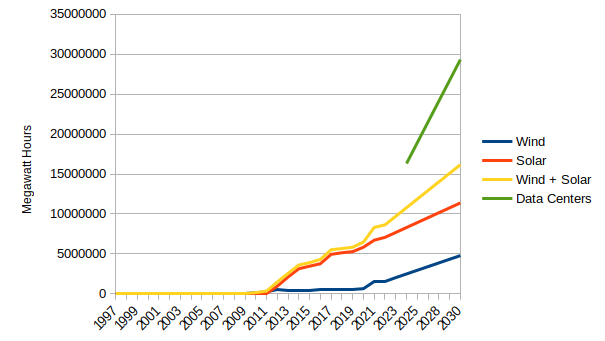
\includegraphics[scale=.75]{projection.png} 
The growth of data centers far outpaces the growth of solar and wind power, which are Arizona’s only significantly expanding renewable energy sources. As shown in the figure, the difference between data center energy use and solar/wind energy production would be about 13.1 million MWh. This discrepancy would have to be met with increased fossil fuel thermoelectric plants. If the difference was made up using natural gas generators, Arizona’s energy production from natural gas would rise by almost 30\%. 

\subsection{Water Sustainability}
Using the same estimates for power as we did to investigate carbon emissions, we estimate that the current water consumption of data centers in Arizona is about 29 billion m\textsuperscript{3}. By 2030, the estimated water consumption of data centers in Arizona is predicted to be 53 billion m\textsuperscript{3}. This would result in an increase to the current water consumption of Arizona by about 6\%. 

\section{Conclusion}
The increasing demand of data centers has led to issues regarding the environmental impact of constructing and running these data centers. Despite concerns, data center demand is expected to nearly double by the end of the decade. In this study, we investigate the sustainability of data center demand in Arizona by predicting future data center growth and comparing it to Arizona's development of greener energy. Our estimates suggest that the rate of development of data centers significantly outpaces Arizona's development of renewable energies, requiring Arizona to nearly triple it's current power production from wind and solar farms by the end of 2030 to match data center development. This is directly at odds with the wider U.S goal of achieving a net-zero carbon emission future. Additionally, the water consumption from data centers in Arizona could lead to further stresses on water supplies in the Southwestern U.S. Due to worsening drought conditions, Arizona can't afford to increase it's current water consumption by nearly 6\%. In order to reliably support the water demand for data centers, Arizona would be required to reduce water in other areas. 
Although innovations in computing efficiency and investments in renewable energy could help reduce the environmental impact of data centers, the current demand growth of data centers in Arizona is unsustainable. More research into how we can incorporate AI into a sustainable future is needed. 


     
\bibliographystyle{plain}
\begin{thebibliography}{99}

\bibitem{GSDemand} Davenport, C. et al (2024). "AI, data centers and the coming US power demand surge". 

\bibitem{DCStats} Data Center Statistics and Map, USA (available at: https://www.datacentermap.com/usa/).

\bibitem{UTDC} Hogan, M. (2015). Data flows and water woes: The Utah Data Center. Big Data \& Society, 2(2). https://doi.org/10.1177/2053951715592429

\bibitem{CloudImpact} Monserrate, Steven Gonzalez. 2022. “The Cloud Is Material: On the Environmental Impacts of Computation and Data Storage.” MIT Case Studies in Social and Ethical Responsibilities of Computing, no. Winter 2022 (January). https://doi.org/10.21428/2c646de5.031d4553.

\bibitem{EnvImpactDC}Siddik, M.; Shehabi, A.; Marston L. (2021). "The environmental footprint of data centers in the United States." Environmental Research Letters, Volume 16, Number 6. https://doi.org/10.1088/1748-9326/abfba1

\bibitem{AZEnergy} U.S. Energy Information Administration, 2023. Arizona Energy Profile (available at: https://www.eia.gov/state/?sid=AZ)

\bibitem{AZDC} Arizona Data Center Size (available at: https://azbigmedia.com/real-estate/phoenix-ranks-as-the-second-largest-data-center-market-in-the-u-s/)

\bibitem{LoadIntensity} Shehabi, A et al. 
"Data center design and location: consequences for electricity use and greenhouse-gas emissions Build. Environ. 46 990–8"

\bibitem{DCPower} Average Power per Area (available at: https://cc-techgroup.com/data-center-energy-consumption/)

\bibitem{DCArea} Arizona Data Center Area (available at: https://azbigmedia.com/real-estate/phoenix-ranks-as-the-second-largest-data-center-market-in-the-u-s/)

\bibitem{DCPUE} Data Center Power Usage Effectiveness (available at: https://www.nrel.gov/computational-science/measuring-efficiency-pue.html)

\bibitem{CoolingEnergy} Shehabi, A et al. (2022). "United States Data Center Energy Usage Report"  https://escholarship.org/uc/item/84p772fc

\bibitem{WaterPerEnergy} National Renewable Energy Laboratory, "Consumptive Water Use for U.S. Power Production." https://www.nrel.gov/docs/fy04osti/33905.pdf

\bibitem{HistoricalData} U.S. Energy Information Administration, Historical State Data (available at: https://www.eia.gov/electricity/data/state/)

\bibitem{c1} 1.	 Yan, M.; Ruan, Z.; Qiu, M. (2007). "Cylindrical Invisibility Cloak with Simplified Material Parameters is Inherently Visible".
\bibitem{c2} Ruan, Z.; Yan, M.; Neff, C. W.; Qiu, M. (2007). "Ideal Cylindrical Cloak: Perfect but Sensitive to Tiny Perturbations". 
\bibitem{c3}Greenleaf, A.; Kurylev, Y.; Lassas, M.; Uhlmann, G. (2007). "Improvement of cylindrical cloaking with the SHS lining".
\bibitem{c4} Yu Luo, Jingjing Zhang, Hongsheng Chen, Bae-Ian Wu, and Jin Au Kong(2007). "A new strategy to conceal an object from electromagnetic wave"


\end{thebibliography}


\end{document}
